\documentclass[a4paper, 11pt]{article}%

%%%%%%%%%%%%%%%%%%%%%%%%%%%%%%%%%%%%%%%%%%%%%%%%%%%%%%%%%%%%%%%%%%%%%%%%

% Global structure parameters
\usepackage{fullpage}%

\usepackage[francais]{babel}%

\usepackage[utf8]{inputenc}%
\usepackage[T1]{fontenc}%

% Font selection
% (newpx n'a pas été installé avex TeXLive...)
\usepackage{mathpazo}%
\usepackage{courier}%

% Macro packages
\usepackage{url}%
\usepackage{graphicx}%
\usepackage{listings}%

\usepackage[font=scriptsize,labelfont=bf]{caption}

% Parameters for listings
\lstset{%
	basicstyle=\footnotesize\sffamily,%
	columns=fullflexible,%
	frame=lb,%
	frameround=fftf,%
	language=caml,%
}%

% Fine tuning
\setlength{\parskip}{0.5\baselineskip}%

%%%%%%%%%%%%%%%%%%%%%%%%%%%%%%%%%%%%%%%%%%%%%%%%%%%%%%%%%%%%%%%%%%%%%%%%

\begin{document}

\title{Rapport de projet}

\author{Marco Freire, Clément Legrand-Duchesne}

\date{26 septembre 2017}

\maketitle

\begin{abstract}
  Dans ce rapport seront expliqués les codes du pavage de Penrose
  suivant différents types de parcours, et des tours de Hanoi, problème
  à contrainte résolu récursivement, ainsi que leurs extensions; et les
  choix d'implémentation que nous avons été menés à faire.
  \begin{description}
    
  \item[Mots-clés:] Pavage; parcours; récursivité; contrainte.

   
%\item[Classification ACM:] Voir les codes à l'adresse
%  \begin{center}
%    \url{http://www.acm.org/about/class/class/2012}.
%  \end{center}

  \end{description}
\end{abstract}

%%%%%%%%%%%%%%%%%%%%%%%%%%%%%%%%%%%%%%%%%%%%%%%%%%%%%%%%%%%%%%%%%%%%%%%%

\section{Penrose}
        \subsection{Principe: algorithme de base}
                Le pavage de Penrose implémenté utilise deux tuiles de
                base, des triangles d'or. Les dimensions de leurs
                côtés sont donc des des nombres flottants. Afin
                d'éviter des erreurs d'arrondi suceptibles de ce
                cumuler, et d'alléger le code, nous avons choisi de ne
                travailler qu'avec des flottants, avant des les
                arrondir en entiers juste avant le tracé.
                
                Par commodité, nous avons suivi la convention
                suivante: les triangles seront représentés par un
                tableau contenant les coordonnées des trois sommets,
                le premier étant celui duquel sont issus les deux
                cotés de longeurs égales, le second est le suivant en
                tournant dans le sens horaire.

                Inserer image!

                Afin de differentier les triangles obtus des triangles
                aigus, nous avons créé un type \texttt{triangle}:

		\begin{lstlisting}
                  type triangle = Obtuse | Acute;;
		\end{lstlisting}

                Une des principales difficultés rencontrées lors de
                l'implémentation de ce pavage est le fait la fonction
                \texttt{fill\_poly} du module \texttt{Graphics.cma}
                remplit le polygone avec une couleur donnée, mais
                recouvre et donc efface les bords de celui ci si ceux
                ci ont été tracés avant. Cela n'est pas encore trop
                contraignant ici, puisqu'il suffit d'écrire la
                fonction \texttt{draw} de la sorte:

                \begin{lstlisting}
                  let draw points triangle =
                      (if triangle = Obtuse then set_color red
                      else set_color blue);
                      fill_poly (iof_array points);
                      move points.(0);
                      set_color black;
                      line points.(1);  
                      line points.(2);
                      line points.(0)
                  ;;
                \end{lstlisting}
                
	\subsection{Améliorations}
		Le premier problème du code précédent est que les
                côtés des triangles sont tous tracés deux fois. Pour y
                remédier, il suffit, lors de chaque subdivision d'un
                triangle, de ne tracer que les séparations entre les
                nouveaux triangles obtenus (et de ne pas oublier les
                cotés du triangle initial).

		Inserer une image! (+ peuve?)

		Il apparaît alors qu'il est necéssaire de tracer ces
                lignes après que les triangles soient remplis, afin
                que celles ci ne soient pas effacées.
		La fonction \texttt{divide} est en réalité un simple
                parcours en profondeur de l'arbre des divisions des triangles.		
		Plutôt que d'afficher directement le pavage, il semble
                plus interressant de montrer la division succéssive
                des triangles pendant la construction du
                pavage. Survient alors une nouvelle difficulté:
                l'algorithme de parcours en profondeur décrit
                précédemment ne convient plus. 
		Une première solution est d'implémenter un parcours
                largeur et de marquer une pause avant d'entamer chaque
                nouvelle profondeur de l'arbre. il faut pour cela
                maintenir une structure de file   En revanche, il est
                alors nettement plus difficle d'afficher les couleurs
                des triangles dessinés à chaque génération et de ne
               tracer chaque coté qu'une seule fois. En effet, à
                chaque nouvelle génération, la coloration des
                triangles efface les cotés de ceux ci si ils ont été
                précédemment tracés. 


\section{Hanoi}

	\subsection{Principe: algorithme de base}
		Le problème des tours de Hanoi est essentiellement récursif. Pour
		déplacer n disques du premier poteau jusqu'au troisième
		il suffit de savoir en déplacer n-1 sur le deuxième poteau (étape 1), puis
		de déplacer le n-ième disque sur le troisième poteau (étape 2) et enfin de
		déplacer encore une fois les n-1 disques sur le troisième poteau (étape 3).

		\begin{figure}[!h]
			\minipage{0.24\textwidth}
			  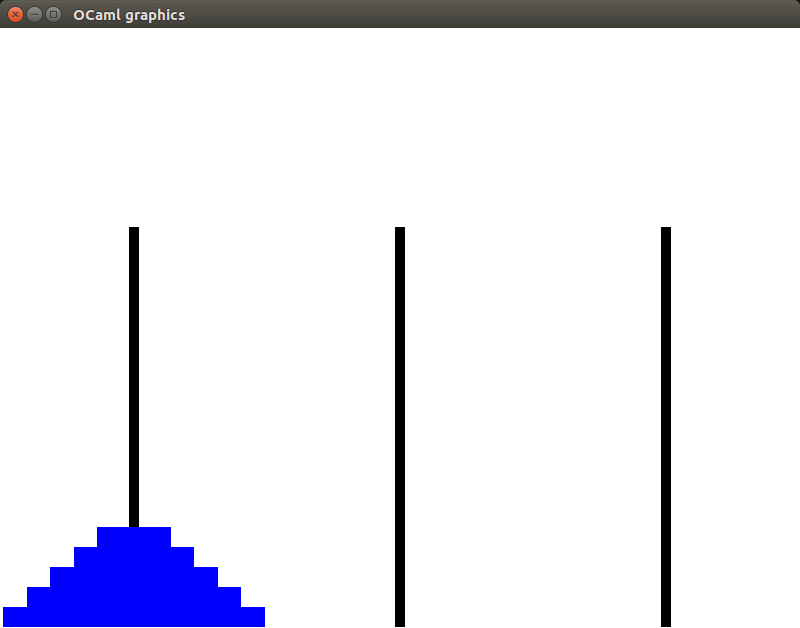
\includegraphics[width=\linewidth]{hanoi_start.png}
			  \caption{État initial}\label{fig:hanoi_start}
			\endminipage\hfill
			\minipage{0.24\textwidth}
			  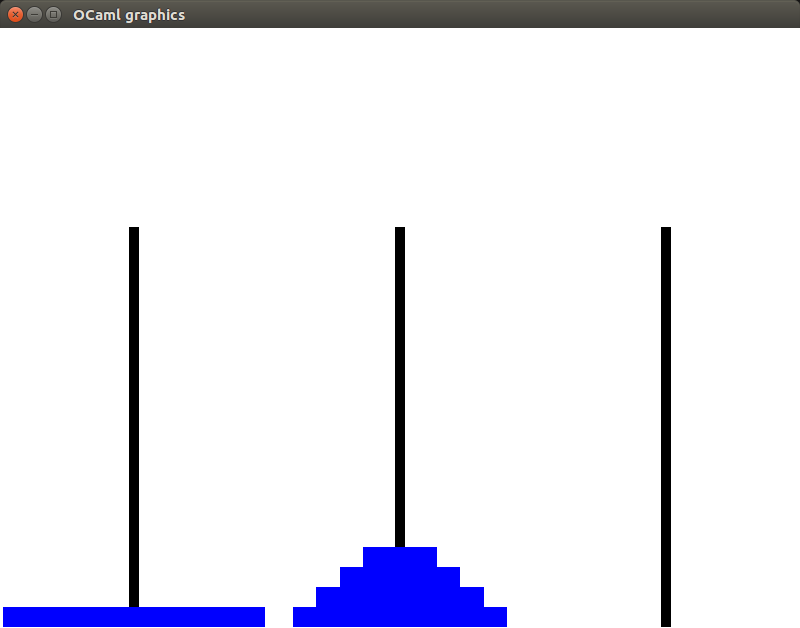
\includegraphics[width=\linewidth]{hanoi_mid1.png}
			  \caption{Fin étape 1}\label{fig:hanoi_mid1}
			\endminipage\hfill
			\minipage{0.24\textwidth}
			  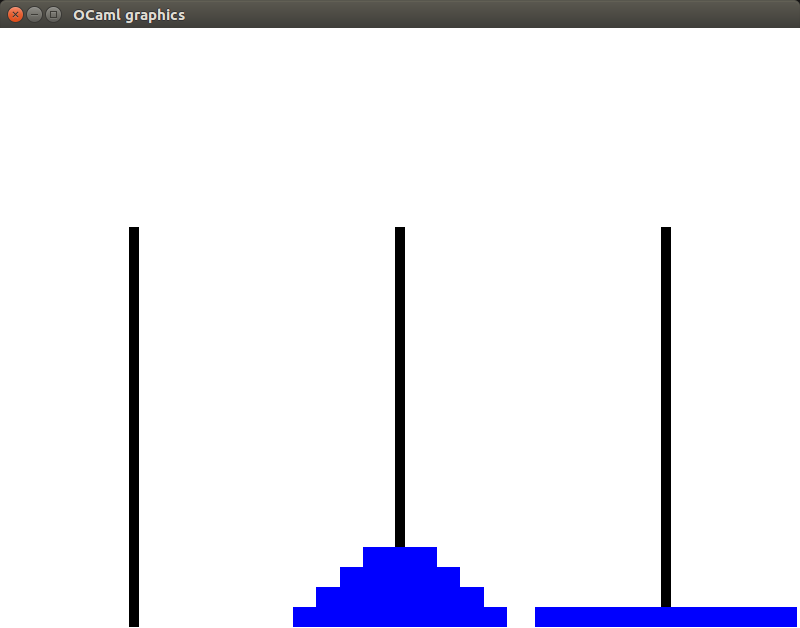
\includegraphics[width=\linewidth]{hanoi_mid2.png}
			  \caption{Fin étape 2}\label{fig:hanoi_mid2}
			\endminipage\hfill
			\minipage{0.24\textwidth}
			  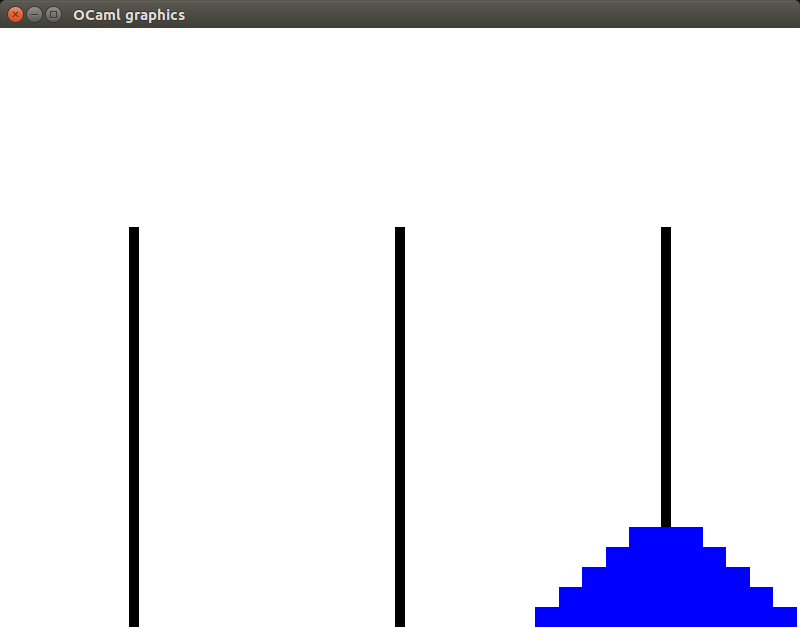
\includegraphics[width=\linewidth]{hanoi_end.png}
			  \caption{État final}\label{fig:hanoi_end}
			\endminipage\hfill
		\end{figure}

		Nous avons choisi pour représenter la situation un tableau de piles
		\texttt{rods}: chaque pile du tableau représente chacun des poteaux et
		contient les disques qui y sont empilés.

		La seule complication du code est le choix du poteau temporaire utilisé
		pour chaque déplacement de disques. La première implémentation réalisée
		repose sur la fonction suivante \texttt{choose}:

		\begin{lstlisting}
		let choose a b =
		  if a = b then failwith "a and b are equal"
		  else if a = 0 then
			if b = 1 then 2
			else 1
		  else if a = 1 then
			if b = 0 then 2
			else 0
		  else if a = 2 then
			if b = 0 then 1
			else 0
		  else failwith "a or b are not between 0 and 2"
		;;
		\end{lstlisting}

		Cette fonction prend en argument deux éléments distincts de {0, 1, 2} et
		renvoie le troisième et est utilisée pour choisir automatiquement dans
		la fonction \texttt{move} le poteau temporaire à utiliser:

		\begin{lstlisting}
		let rec move rods num_discs orig_rod dest_rod =
		  if num_discs = 1 then
			  move_disc rods orig_rod dest_rod
		  else
			(
			  let temp_rod = choose orig_rod dest_rod in
			  move rods (num_discs - 1) orig_rod temp_rod;
			  
			  move_disc rods orig_rod dest_rod;
			  
			  move rods (num_discs - 1) temp_rod dest_rod;
			)
		;;
		\end{lstlisting}

		Lors de l'implémentation de la fonction résolvant le problème des tours
		de Hanoi à n poteaux, nous nous sommes rendu compte que la fonction
		\texttt{choose} était difficilement généralisable. Nous avons donc choisi
		de passer le poteau intermédiaire en argument à la fonction \texttt{move}.

		Cette modification permet de choisir comme l'on veut le poteau intermédiaire,
		ce qui est nécessaire pour la version généralisée de l'algorithme.
	
	\subsection{Analyse du problème}
		
		Il est possible de calculer le nombre minimal de déplacements à effectuer
		pour résoudre le problème.
		
		Si l'on veut déplacer n disques du premier piquet au dernier, il
		faut nécessairement déplacer le plus grand. Or il n'est possible
		de le déplacer que si les (n-1) disques plus petits ne sont pas
		sur celui-ci. Puisque l'on veut déplacer le plus grand disque sur
		le dernier piquet, les (n-1) disques doivent se trouver empilés
		en ordre décroissant de taille sur le piquet central; dans quel
		cas on peut déplacer le grand disque sur le dernier poteau, et
		déplacer encore les autres disques sur le dernier piquet.
		
		On a ainsi la relation de récurrence suivante, qui se résout facilement:
		
		\begin{description}
			\item[Initialisation] $M(1) = 1$
			\item[Relation de récurrence] $M(n) = 2M(n-1) + 1$
			\item[Relation générale] $M(n) = 2^n - 1$
		\end{description}
		
		Le nombre de déplacements de disques effectués pas l'algorithme
		dans le cas où il n'y a que trois piquets est optimal.
				
		\begin{figure}[!h]
			\minipage{0.49\textwidth}
			  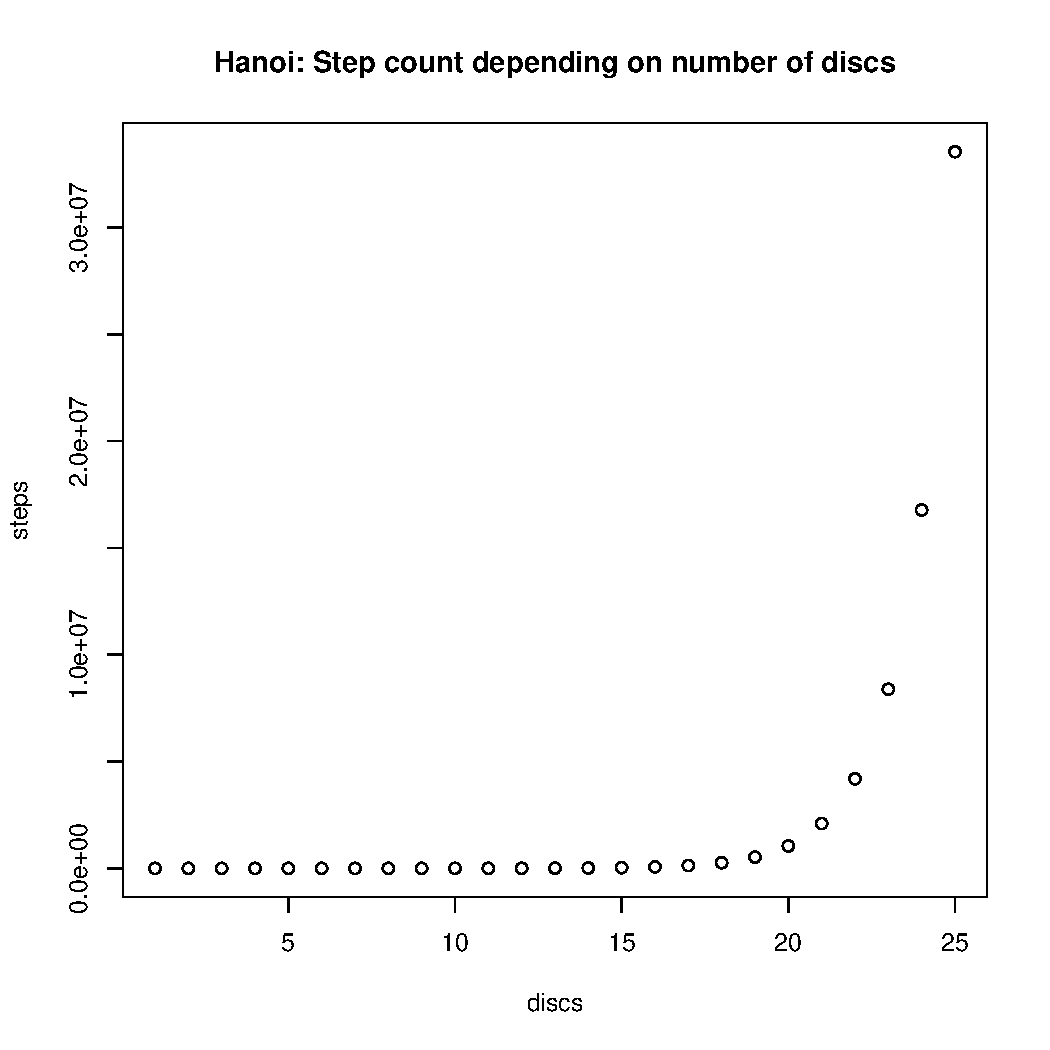
\includegraphics[width=\linewidth]{steps_plot.pdf}
			\endminipage\hfill
			\minipage{0.49\textwidth}
			  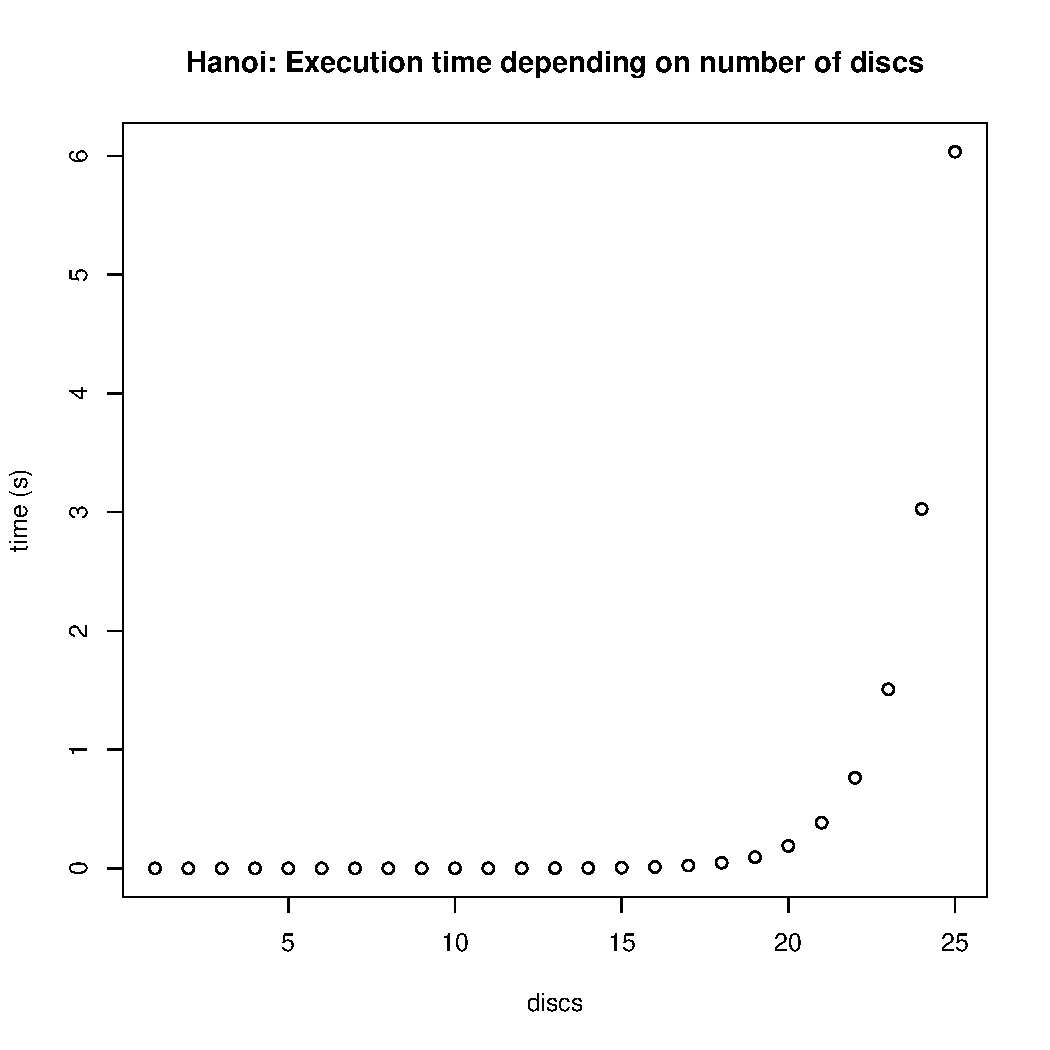
\includegraphics[width=\linewidth]{time_plot.pdf}
			\endminipage\hfill
		\end{figure}
			
		Les résultats expérimentaux sont en accord avec
		le calcul théorique: le nombre de mouvements
		est fonction exponentielle du nombre
		initial de disques.
	
	\subsection{Principe: algorithme généralisé}
		Pour ce problème, l'implémentation choisie est la deuxième présentée.
		
		Cette fois il s'agit d'utiliser au mieux les poteaux supplémentaires.
		Nous avons calculé le nombre de disques pouvant être sur les poteaux
		intermédiaires, pour répartir ces disques sur chacun des poteaux intermédiaires
		en utilisant comme poteau temporaire le dernier (étape 1), ensuite il faut
		déplacer le disque le plus grand sur le dernier poteau (étape 2), et finalement
		il suffit de réaliser le parcours inverse de celui effectué dans l'étape 1,
		et de regrouper les disques intermédiaires sur le dernier poteau (étape 3).
		
		\begin{figure}[!h]
			\minipage{0.24\textwidth}
			  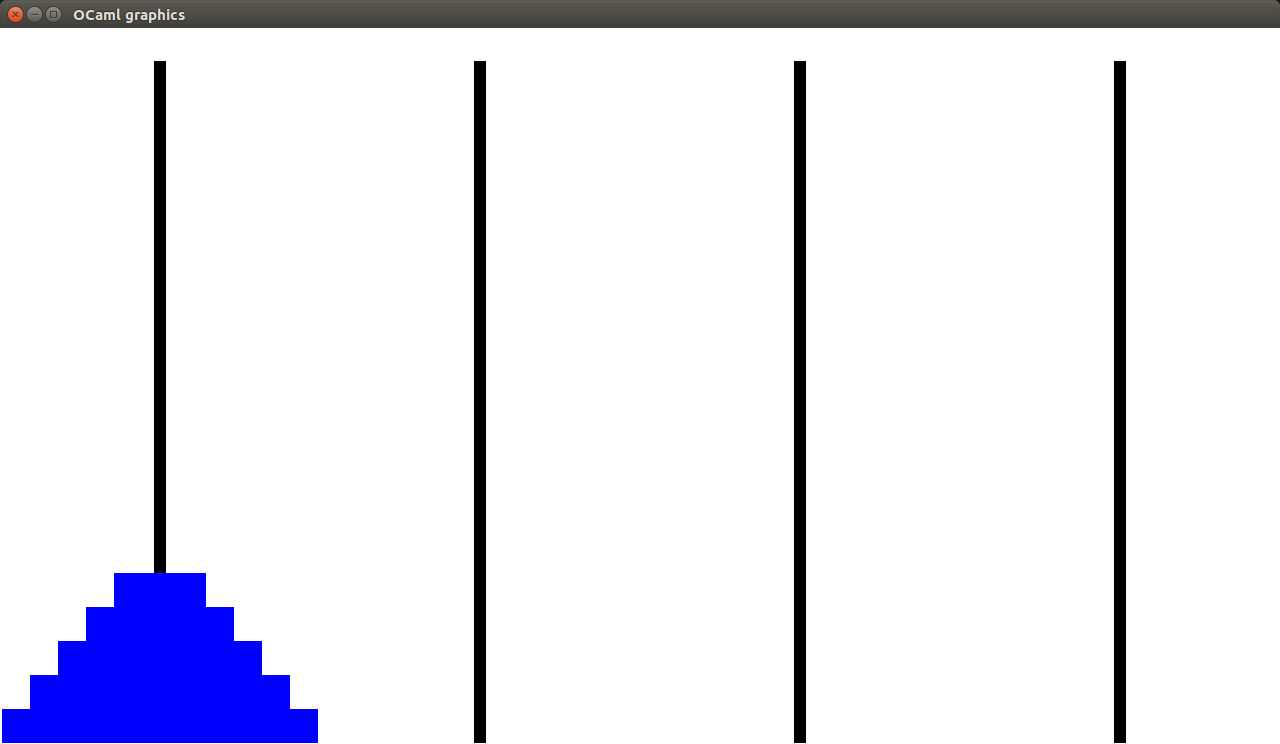
\includegraphics[width=\linewidth]{hanoi_gen_start.png}
			  \caption{État initial}\label{fig:hanoi_gen_start}
			\endminipage\hfill
			\minipage{0.24\textwidth}
			  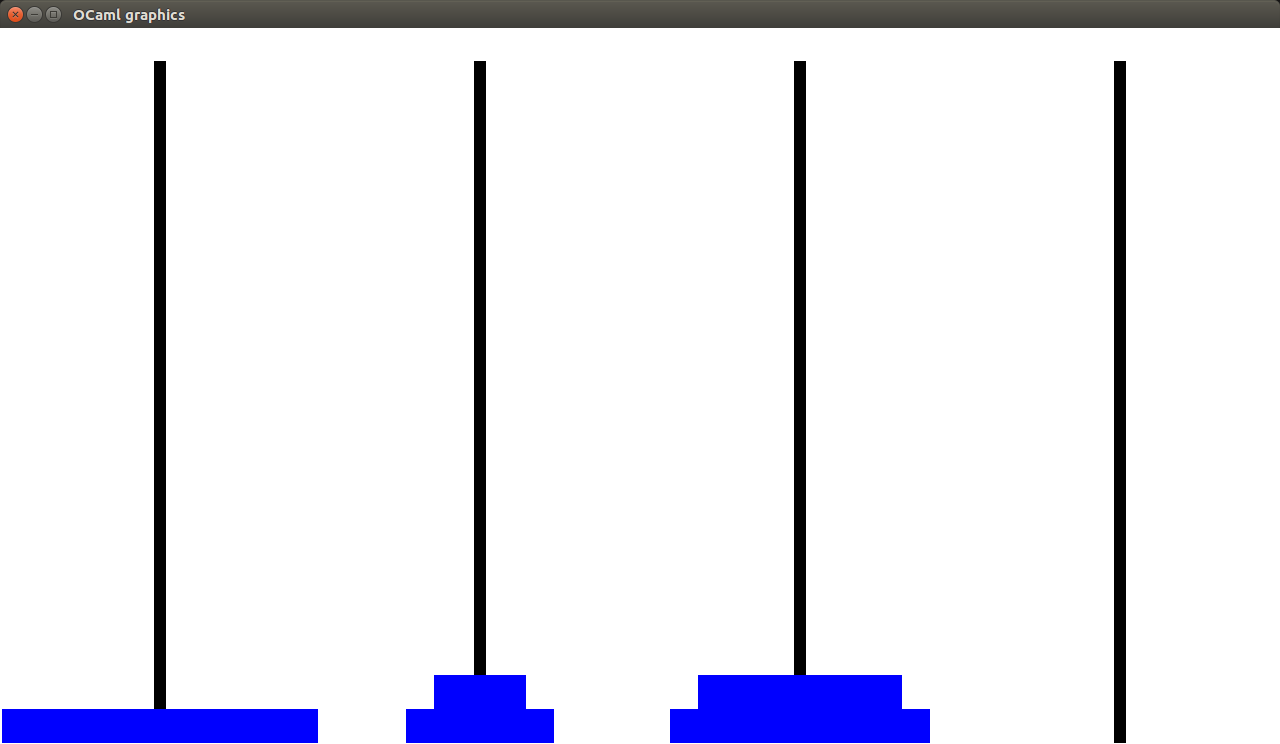
\includegraphics[width=\linewidth]{hanoi_gen_mid1.png}
			  \caption{Fin étape 1}\label{fig:hanoi_gen_mid1}
			\endminipage\hfill
			\minipage{0.24\textwidth}
			  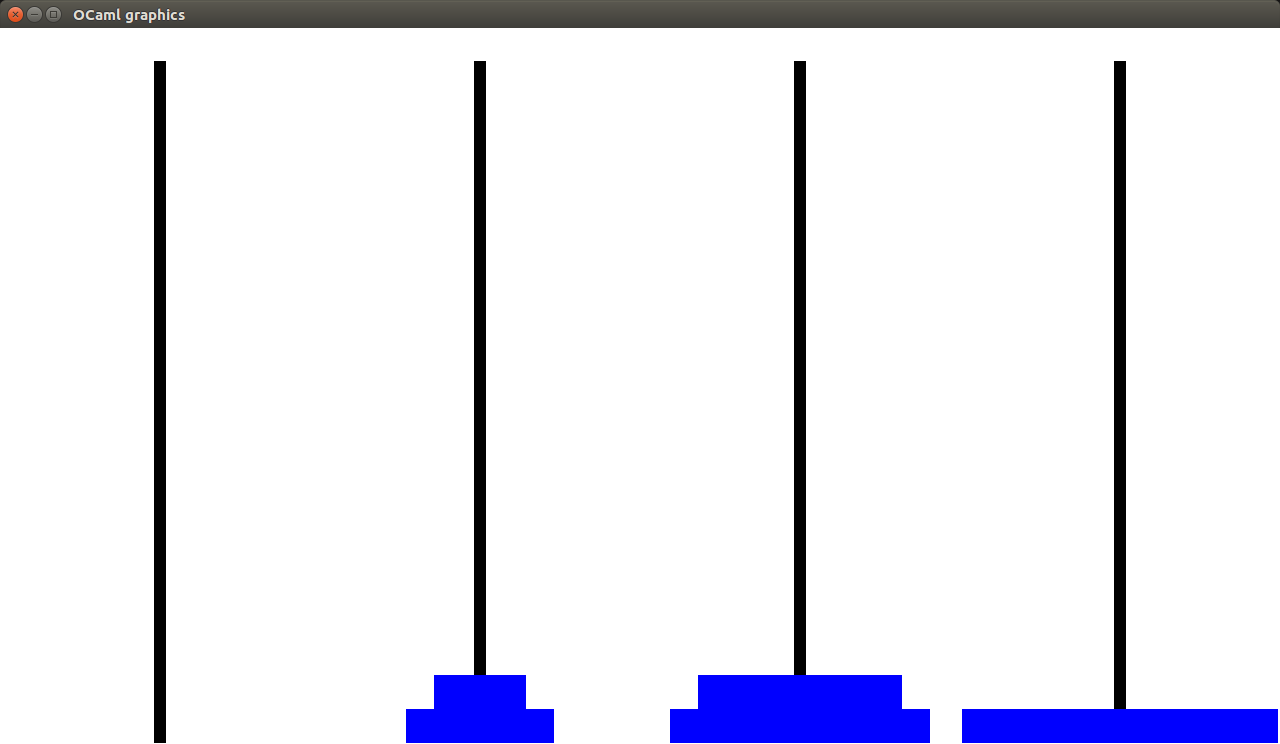
\includegraphics[width=\linewidth]{hanoi_gen_mid2.png}
			  \caption{Fin étape 2}\label{fig:hanoi_gen_mid2}
			\endminipage\hfill
			\minipage{0.24\textwidth}
			  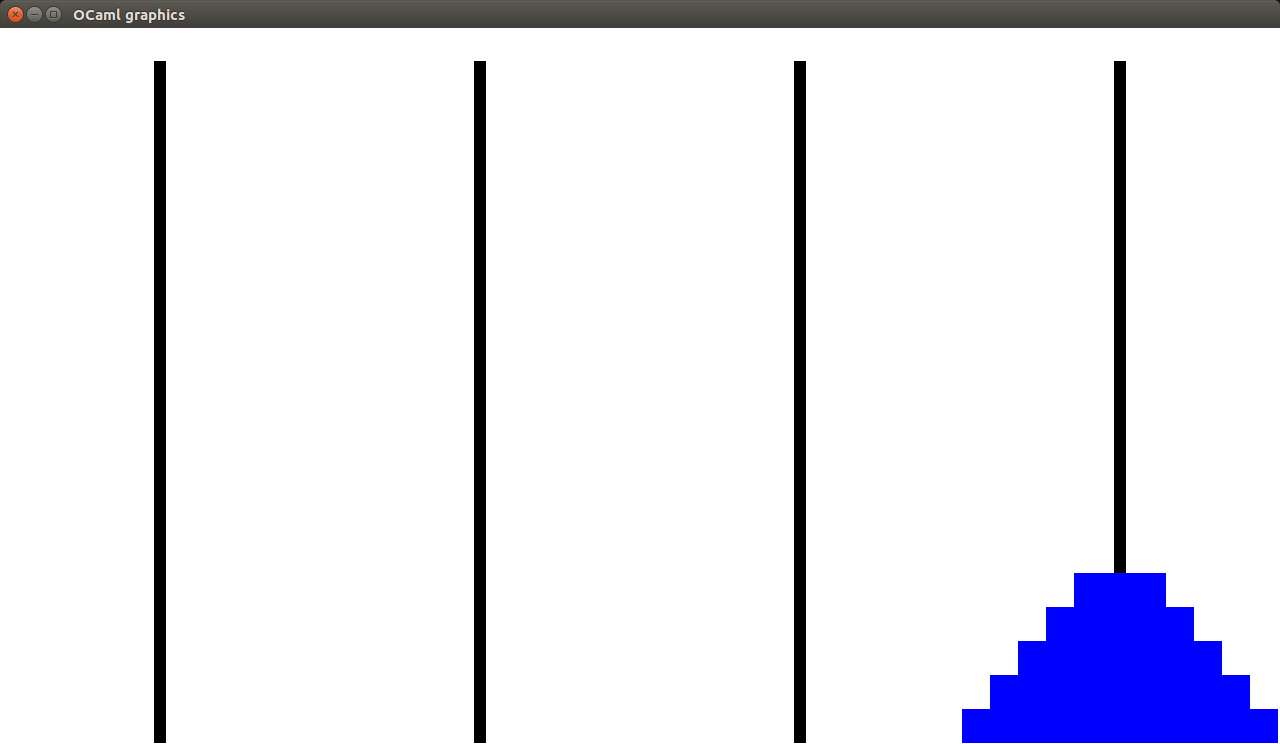
\includegraphics[width=\linewidth]{hanoi_gen_end.png}
			  \caption{État final}\label{fig:hanoi_gen_end}
			\endminipage\hfill
		\end{figure}
		
		Ainsi beaucoup moins de déplacements sont nécessaires pour la résolution
		du problème.
	
	\subsection{Affichage}
		Nous avons créé un affichage grâce au module \texttt{Graphics}
		de OCaml qui permet de visualiser la résolution du problème à n
		disques et p poteaux pour n et p raisonnables.
		
		\begin{figure}[!h]
			\minipage{0.49\textwidth}
			  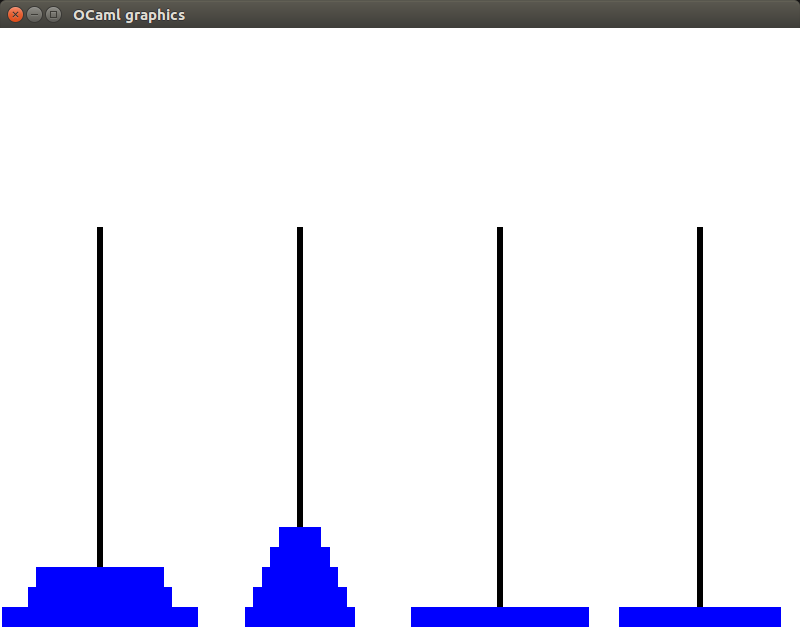
\includegraphics[width=\linewidth]{hanoi_10_4.png}
			  \caption{Affichage de \texttt{hanoi 10 4}}
			\endminipage\hfill
			\minipage{0.49\textwidth}
			  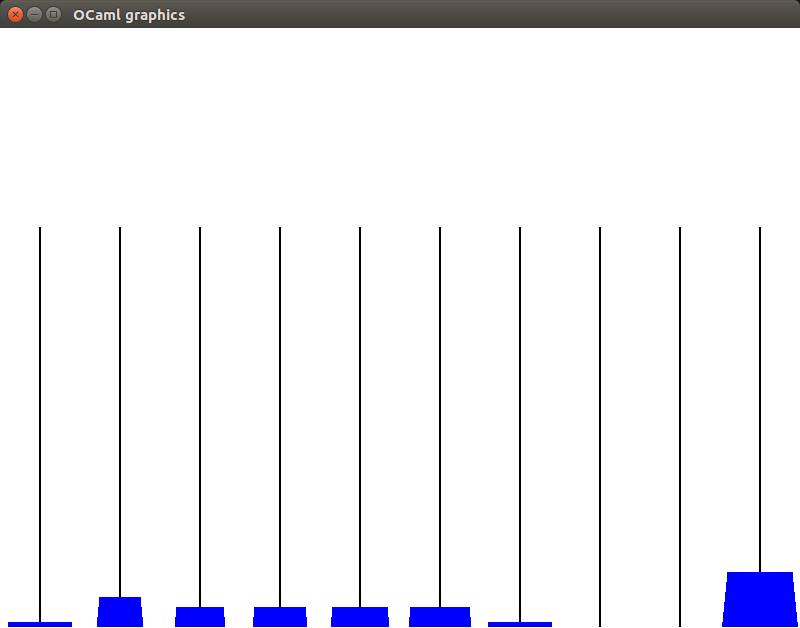
\includegraphics[width=\linewidth]{hanoi_35_10.png}
			  \caption{Affichage de \texttt{hanoi 35 10}}
			\endminipage\hfill
		\end{figure}
		
		De plus l'affichage s'adapte à la taille de la fenêtre:
		
		\begin{figure}[!h]
			\minipage{0.49\textwidth}
			\begin{center}
			  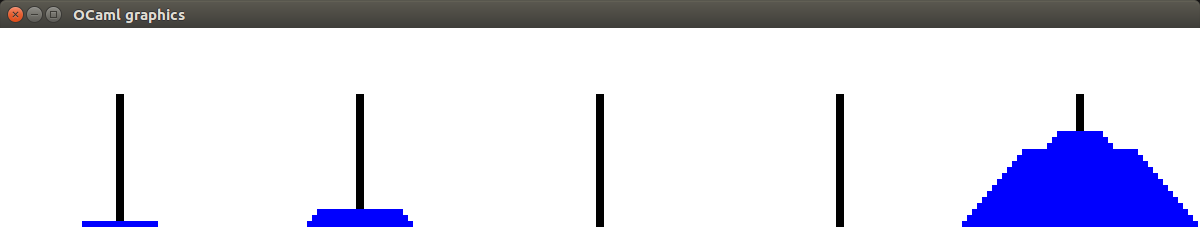
\includegraphics[width=7cm]{hanoi_wide.png}
			  \caption{1200 x 200}
			\end{center}
			\endminipage\hfill
			\minipage{0.49\textwidth}
			\begin{center}
			  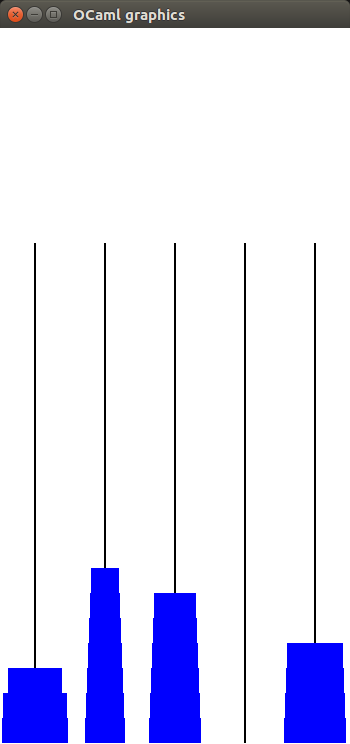
\includegraphics[height=5cm]{hanoi_tall.png}
			  \caption{350 x 750}
			\end{center}
			\endminipage\hfill
		\end{figure}
	
		La taille des disques est donc variable et dépend de plusieurs
		facteurs: au moins il y a de poteaux et au plus la fenêtre est
		large, au plus les disques sont larges; au plus il y a de disques
		et au plus la fenêtre est grande, au plus les disques sont hauts.
	
	\subsection{Améliorations}
		Nous nous sommes rendus compte qu'il était possible d'améliorer
		l'algorithme généralisé, puisqu'on observe que à chaque fois
		qu'un pile de disques est déplacée, seul le premier ou le dernier
		piquet est utilisé comme piquet temporaire, alors que l'on dispose
		de plusieurs piquets libres.
	
\section*{Conclusion}

	\begin{itemize}
		\item Nous avons implémenté le programme dessinant le pavage de
		Penrose, à l'aide d'un parcours en profondeur ou d'un parcours
		en largeur, avec la possibilité d'utiliser une homothétie pour
		agrandir la figure à chaque génération; puis le programme résolvant
		le problème des tours de Hanoi simple et généralisé, avec affichage
		graphique.
		%\item Ce que vous avez choisi de ne pas faire.
		\item Il serait intéressant d'implémenter pour les pavages de Penrose
		une version où l'un des triangles serait fixe au cours des générations
		afin de créer l'illusion de la construction du motif autour d'un
		seul triangle.
		Pour les tours de Hanoi, il serait possible de corriger l'algorithme
		généralisé et utiliser tous les piquets libres à notre disposition
		afin de résoudre le problème en moins de déplacements.
	\end{itemize}

\appendix

\section*{Auto-Évaluation}

	%Votre auto-évaluation selon le schéma SWOT/FFOM~(\url{https://fr.wikipedia.org/wiki/SWOT}).
	\begin{description}
		\item[Forces.] En ce qui concerne la partie consacrée au Tours de Hanoi
		je pense que le point fort est l'affichage très flexible que nous avons
		implémenté.
		\item[Faiblesses.]  Le manque de modularité et de séparation du code
		s'est vu très pénible au moment d'harmoniser les différentes versions
		du code à envoyer (algorithme basique, généralisé et avec affichage).
		\item[Opportunités.] Ce projet m'a appris l'importance de la modularité
		du code, pour les raisons avant mentionnées, et aussi à gérer un projet
		mené par plusieurs personnes, ce qui peut s'avérer plus difficile que
		prévu.
		\item[Menaces.] Il est trop souvent facile de remplir le code de
		littéraux et de constantes, mais quand il faut généraliser le
		code déjà écrit, cet effort non effectué fait perdre énormément de temps.
	\end{description}
	
\end{document}

%%%%%%%%%%%%%%%%%%%%%%%%%%%%%%%%%%%%%%%%%%%%%%%%%%%%%%%%%%%%%%%%%%%%%%%%
